\subsection{Rangefinder Testing}
The URG-04LX scanning laser rangefinder requires an external 5V power source connection. With the power connected and the device on, the device is ready and waiting for communication.

\subsubsection{Testing via the Data Viewing Tool}
The URG-04LX has a data viewing tool which is a useful application by Hokuyo Automatic Co. that can be used to view, record, and replay the device's data. To use this tool the device must be plugged into a computer via its USB port. Figure \ref{URGBenriStandard_pic} below shows a screen capture of the application recording data captured by the rangefinder.

\begin{figure}[H]
	\centerline{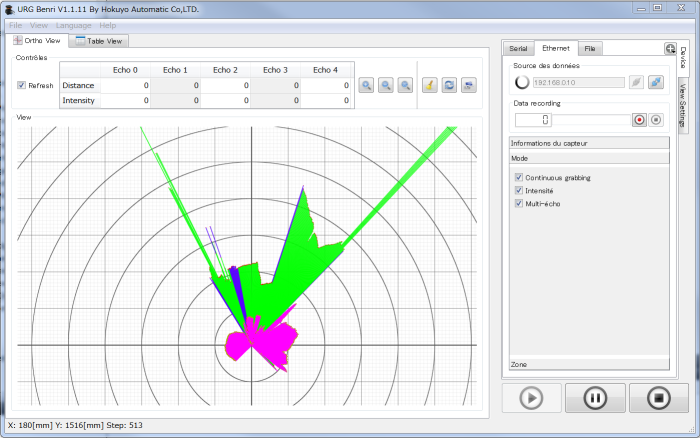
\includegraphics[width=1\textwidth]{UrgBenri_screenshot.png}}
	\caption{Screen Capture of the URG-04LX Data Viewing Tool \cite{URGBenriStandard_ref}}
	\label{URGBenriStandard_pic}
\end{figure}

Note that the start point of 0, end point of 768, and dead zone align to that shown in Figure \ref{rangefinder_fov}. For this project the data viewing tool was used to verify our project's data processing functionality.

\subsubsection{Command Testing}
In addition to the dat viewing tool, we were able to test the rangefinder's commands by connecting it to a laptop via its USB port. We used PuTTy, a serial console application, to communicate with the rangefinder. Figure \ref{rangefinder_putty} shows the data transfer via PuTTy between a laptop and the rangefinder. Note that PuTTy only shows data received, and that the rangefinder always echoes back the command that it receives.

\begin{figure}[H]
	\centerline{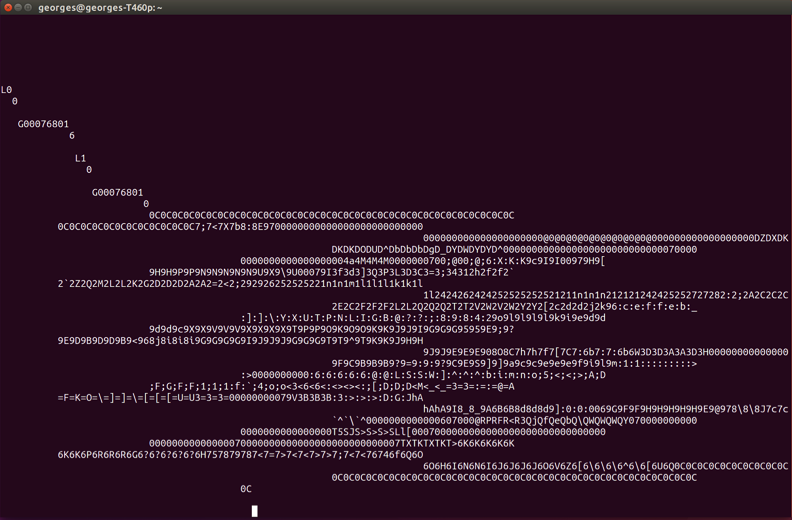
\includegraphics[width=1\textwidth]{rangefinder_putty.png}}
	\caption{Rangefinder Communication Test via PuTTy}
	\label{rangefinder_putty}
\end{figure}

The figure above shows four communication sequences. The first is the laser illumination command 'L0\textbackslash{}n'. Since the laser defaults on, this command turned the laser off. The rangefinder responded to this command first with the echo 'L0\textbackslash{}n', and then with '0', indicating success. The second command is our data acquisition command 'G00076801\textbackslash{}n'. The rangefinder responded with '6', indicating an error code, which was caused by the laser being off. The third command is the laser illumination command again, which turns on the laser. The rangefinder's response was '0' again, indicating success. The last command shown is the data acquisition command again. The rangefinder's response begins with '0', indicating success, followed by the distance data block. The data block consists of 768 points, specified by the data acquisition command. Each data point consists of two characters \cite{urg04lx_datasheet}. By communicating with the rangefinder via PuTTy, we were able to observe the rangefinder's behavior and confirm the data acquisition command functions properly. This testing also verified that communication via the rangefinder's USB port was working.

\subsubsection{Communication via USB On-The-Go (OTG)}
With communication via the rangefinder's USB port working, we decided to continue with this mode of communication. The ZedBoard supports USB OTG which is a specification that allows USB devices to act as a host for other USB devices \cite{usb-otg}. With USB OTG, a device can choose to act as a peripheral or a host if necessary. For the purpose of this project, the ZedBoard will act as the host by initiating communication with the rangefinder. Enabling USB OTG can be done in the Zynq7 Processing System and controlled through the PS. The rangefinder's laser illumination command was chosen to be transmitted from the ZedBoard to test the communication. This command was chosen because when received, the status LED on the rangefinder blinks until the laser is turned back on, which is a simple way of verifying successful communication. In addition, when a command is transmitted via UART from the ZedBoard, its TX LED flashes. A fully successful transaction would observe the ZedBoard's TX LED flashing and then the status LED on the rangefinder blinking.
\par
The ZedBoard was programmed, the rangefinder was turned on, and the two devices were connected by a standard micro-USB to mini-USB cable. The ZedBoard transmitted the command, as signified by the blink of the TX LED. However the rangefinder did not acknowledge the command; its status LED was staying lit signifying the laser was on. Due to this failure\footnote{This communication failure was most likely due to the lack of necessary hardware, as USB OTG requires an adapter that controls which device will be hosting the communication. Without this adapter, both USB devices will act as a peripheral, and neither will initiate communication \cite{usb-otg}.}, using USB OTG was not implemented. Instead the methodology described in Section \ref{sssec:rangefinder_communication} was implemented.

\subsubsection{Communication via Pmod}
Once we decided not to continue with USB OTG, we routed the UART signals to a Pmod connector, described in Section \ref{sssec:rangefinder_communication}. To make sure that UART via Pmod was functioning correctly, the transmit pin was measured with an oscilloscope. The laser illumination command "L0\textbackslash{}n" was transmitted and observed indicating success, as shown in Figure \ref{laser_illumination}. Note that this is a TTL signal.

\begin{figure}[H]
	\centerline{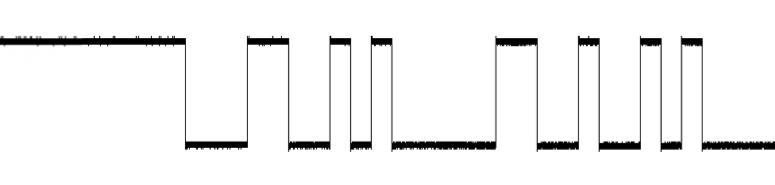
\includegraphics[width=.7\textwidth]{laser_illumination.png}}
	\caption{Laser Illumination Command TTL Oscillogram}
	\label{laser_illumination}
\end{figure}

The RS-232 to TTL converter with the attached breakout board was attached to the ZedBoard. The converter's V\textsubscript{CC} and GND were connected to the ZedBoard Pmod's respective V\textsubscript{CC} and ground pins. When these pins were connected, the converter's power LED turned on. In addition, the converter's RX and TX pins were connected to the ZedBoard's respective TX and RX pins. The breakout board's TX pin was measured on the oscilloscope to observe the resultant RS-232 waveform. However when the command was transmitted from the ZedBoard, there was no change on the oscilloscope. We disconnected the converter's TX and RX pins and reconnected them such that the converter's RX and TX pins were connected to the ZedBoard's respective RX and TX pins. The laser illumination command was re-transmitted and the waveform in Figure \ref{rangefinder_rs232} was observed on the oscilloscope. The oscillogram shows a waveform from +6V to -6V, which is a valid RS-232 signal.

\begin{figure}[H]
	\centerline{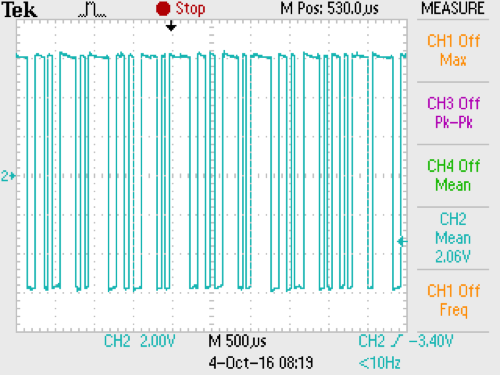
\includegraphics[width=.7\textwidth]{rangefinder_rs232.png}}
	\caption{Laser Illumination Command RS-232 Oscillogram}
	\label{rangefinder_rs232}
\end{figure}

With the communication functioning properly, the rangefinder's RX and TX were connected to the breakout board's respective TX and RX pins, and the laser illumination command was transmitted from the ZedBoard. The rangefinder's status LED started blinking, signifying that it received the laser illumination command and the laser was turned off. This test's success indicates that the rangefinder's communication is completely successful.

\subsubsection{PS-PL Testing}
%talk about transmitting the command from the button press -> uart led blinking
%testing vga stuff



